\section{Grundlagen}
In den Grundlagen wird ein Überblick zum Aufbau des Systems und der Software des Tankautomaten gegeben. Ebenfalls soll näher auf das OCPP Protokoll und das damit zusammenhängende WebSocket Protokoll eingegangen werden. Diese bilden die Basis für die spätere Planung, Umsetzung und Testung der Protokollintegration.
\subsection{Tankautomat}
Das System besteht, wie bereits in der Einleitung kurz erwähnt aus dem Tankautomaten, den damit verbundenen Stationen und dem Cloudserver über den die Weboberfläche gehostet wird. Diese Zusammenhänge sind in \autoref{fig:Systemübersicht} dargestellt. Sie werden im Zuge des Abschnittes nach und nach erläutert. Dabei muss zuerst verstanden werden, wie der bisherige Tankablauf adaptiert werden kann. Hierfür muss in diesem Kapitel zuerst genauer auf die Mechaniken im Tankautomaten eingegangen werden.

\begin{figure}[H]
	\centering
	\includegraphics[width=0.6\textwidth]{images/System/Systemübersicht.png}
	\caption{Systemübersicht des Tankautomaten\cite{Eigene_Darstellung}}
	\label{fig:Systemübersicht}
\end{figure}
%Um die Abläufe im System zu verstehen muss zuerst der Aufbau der Betriebstankstelle erläutert werden. In \autoref{fig:Systemübersicht} sind alle Akteure der Betriebstankstelle zusehen und wie diese miteinander agieren.
%%Abbildung anpassen: Pfeil Web interface mit weboberfläche ersetzen, zw. cloud und BTS3 API hinzufügen.

%\noindent Das \acs{BTS3} Terminal ist der zentrale Akteur im Aufbau. Bei dem Terminal handelt es sich um ein ARM basiertes System. Als Betriebssystem wird Linux genutzt. Zur Bedienung des Tankautomaten wird ein Touch-Display verwendet. Weiter besitzt es unter anderem:
%\begin{itemize}
% \item Eine Ethernet Schnittstelle zur Kommunikation mit der \textit{Cloud}.
% \item 8 Impulseingänge zur Zählung der gesendeten Impulse über die Impulsschnittstelle.
% \item 8 $I^{2}C$ Eingänge zur Erkennung der Zapfpistolen Entnahme.
% \item 8 Relais zur Zapfsäulenfreischaltung.
% \item Ein \ac{RFID} Lesegerät.
%\end{itemize}
%\noindent Sowie andere Sensoren auf die hier nicht genauer eingegangen wird. \\
%Die \textit{Cloud} dient als Verwaltungstool, das über eine Weboberfläche von einem beliebigen Endgerät erreichbar ist. Hier können angeschlossene Geräte konfiguriert werden, Freigaben für Fahrer sowie Fahrzeuge festgelegt werden, Softwareupdates durchgeführt und abgeschlossene Tankvorgänge eingesehen werden. Die Konfigurationsparameter und Freigaben werden in einer Datenbank abgespeichert.\newline

\subsubsection{Tankablauf}
Als Erstes muss der typische Tankablauf am Tankautomat erläutert werden, die als Basis für den Ladevorgang dienen soll. Dieser beginnt, nachdem der Fahrer mit seinem Fahrzeug am Einsatzort des Tankautomaten eintrifft. Der Fahrer begibt sich daraufhin zum Tankautomat und weist sein Fahrzeug mit einer Identifikationsnummer oder mithilfe eines \acs{RFID} Chips am Tankautomat nach. Danach wird er aufgefordert, die aktuelle Laufleistung des Fahrzeuges anzugeben und muss sich danach selbst mit einer Nummer identifizieren. Nach erfolgreicher Identifikation öffnet sich die Produktauswahl. Hier kann er nun alle am Tankautomaten verbundenen Stationen einsehen, für die er und sein Fahrzeug freigegeben sind. Wird jetzt eine Station ausgewählt, wird über ein Freigabe Relais im Tankautomaten, die Pumpe an der Zapfsäule aktiviert. Dabei wird auf dem Display in eine Übersicht mit allen anderen aktiven Tankvorgängen gewechselt. Jetzt kann der Fahrer die Zapfpistole aus der Zapfsäule entnehmen und sein Fahrzeug tanken. Während des laufenden Tankvorgangs wird die getankte Menge in der Übersicht angezeigt. Die getankte Menge erhält der Tankautomat über einen Impulsgeber in der Zapfsäule, der proportional zur Flüssigkeitsmenge, eine Impulsfolge ausgibt (vgl. \cite{Patent_Zapfsauele}). Sobald das Fahrzeug vollgetankt ist oder ein Limit erreicht wurde, kann die Zapfpistole wieder in die Zapfsäule eingesteckt werden. Nachdem einstecken wird der Tankvorgang beendet und die finale Tankmenge für weitere 60 Sekunden auf dem Display angezeigt. Diese Transaktion wird währenddessen auf den Cloudserver, mit allen zuvor angegeben Daten, hochgeladen. Diese können dann über die Weboberfläche eingesehen werden.\newline

\noindent Neben diesem Tankablauf existiert ein gesonderter Ablauf, falls nur eine Station am Tankautomat angeschlossen ist. Dabei wird nach der Fahreridentifikation, die Produktauswahl übersprungen und direkt die Freigabe an der einzigen Station erteilt.

\subsubsection{Cloud Schnittstelle}
Die in der Cloud gesetzten Einstellungen werden über eine \acfi{API} zyklisch mit dem Tankautomat synchronisiert. Hierfür wird alle 60 Sekunden der aktuelle Stand mit dem Cloudserver ausgetauscht. Auf Basis dieser Daten werden die im Ablauf erklärten Freigaben, Limits und Stationsauswahlen geregelt. Es ist auch möglich, das Terminal im Offline Modus zu betreiben. In diesem wird mit dem zuletzt übertragenen Stand an Berechtigungsdaten und Stationsdaten gearbeitet. Abgeschlossene Transaktionen werden hier zwischengespeichert und werden, sobald die Verbindung zum Cloudserver wiederhergestellt ist, übertragen. Dabei werden ebenfalls die neuen Berechtigungs- und Stationsdaten empfangen.

\subsubsection{Lokaler Datenbankspeicher}
Die von der Cloud geteilten Einstellungen werden lokal auf dem Tankautomaten gespeichert. Hierfür wird eine lokale Datenbank genutzt. In dieser werden in Tabellen neben den Freigabe- und Stationsdaten ebenfalls die getätigten Transaktionen zwischengespeichert, die an den Cloudserver gesendet werden. Von besondere Bedeutsamkeit ist für diese Arbeit die Stationen Tabelle. Der Aufbau dieser ist in \autoref{tab:Datenbank_Tabelle_Stations} zu sehen.
\begin{table}[H]
	\begin{center}
		\begin{tabular}{|ll|}
			\hline
			\multicolumn{2}{|l|}{\textbf{Stations}} \\ \hline
			\multicolumn{1}{|l|}{id} & TEXT \\ \hline
			\multicolumn{1}{|l|}{number} & TEXT \\ \hline
			\multicolumn{1}{|l|}{isLocked} & INTEGER \\ \hline
			\multicolumn{1}{|l|}{isLockLevelLocked} & INTEGER \\ \hline
			\multicolumn{1}{|l|}{lockLevel} & INTEGER \\ \hline
			\multicolumn{1}{|l|}{currentLockLevel} & INTEGER \\ \hline
			\multicolumn{1}{|l|}{limitTransaction} & INTEGER \\ \hline
			\multicolumn{1}{|l|}{isOnStorage} & INTEGER \\ \hline
			\multicolumn{1}{|l|}{counter} & INTEGER \\ \hline
			\multicolumn{1}{|l|}{productId} & TEXT \\ \hline
			\multicolumn{1}{|l|}{storageId} & TEXT \\ \hline
			\multicolumn{1}{|l|}{hwMode} & TEXT \\ \hline
			\multicolumn{1}{|l|}{hwChannel} & INTEGR \\ \hline
			\multicolumn{1}{|l|}{type} & TEXT \\ \hline
			\multicolumn{1}{|l|}{impulseRate} & INTEGER \\ \hline
		\end{tabular}
	\end{center}
	\caption{Aufbau der Datenbanktabelle \glqq{}Stations\grqq{} \cite{Eigene_Darstellung}}
	\label{tab:Datenbank_Tabelle_Stations}
\end{table}

\noindent Neben vieler anderer Felder, sind hier das Feld \glqq{}type\grqq{} und \glqq{}hwChannel\grqq{} gespeichert.
Über das Feld \glqq{}type\grqq{} wird die Schnittstelle angegeben, mit der die Station mit dem Tankautomaten kommuniziert. Der einzige existierende Wert hierfür war zu Beginn der Arbeit: \glqq{}IMPULSE\grqq{}. Neben diesem wird mit dem \glqq{}hwChannel\grqq{} angegeben, an welchem Pumpenfreigaberelais die Zapfsäule angeschlossen ist. Die Bedeutung der Felder wird später zum Verständnis der Konzeption und Umsetzung benötigt.
\subsection{Software}
Die in der Softwareentwicklung des Projekt \glqq{}Tankautomaten\grqq{} genutzte Programmiersprache ist \cpp. Die verwendete Version ist \cpp 11. Neben \cpp wurde auch das Qt-Framework zur Entwicklung genutzt.
\subsubsection{Qt Framework}
Auf der Basis von \cpp wurde das Qt Framework entwickelt. Es handelt sich dabei um eine Sammlung von Bibliotheken, die zur Entwicklung Plattform übergreifenden Applikationen genutzt werden (vgl. \cite{Qt-about}, \glqq{}What is Qt?\grqq{}). Es unterstützt viele Plattformen und ist auf den bekannten wie z. B. Windows, Linux, Android, etc. verfügbar. Qt erweitert dabei \cpp mit eigenen Funktionen, wie z. B. den \textit{signals and slots}. Dieser Mechanismus erlaubt es \textit{callback} Funktionen zu ersetzen. Dabei wird bei einem Event ein Signal ausgestrahlt, das einen Slot aufruft(vgl. \cite{Qt-signals-and-slots}, \glqq{}Signals and Slots\grqq{}). Das Framework wurde in der Version 5.15 genutzt. Das Qt-Framework kommt ebenfalls mit einer eigenen JavaScript basierten Sprache zur Erstellung visueller Komponenten namens \acfi{QML}. Diese wurde neben \cpp zur Entwicklung des \acfi{GUI} im Tankautomaten genutzt.
\subsubsection{Qt Test}
Zum Testen der Applikation wurde bisher das Qt Test Framework genutzt. Dabei handelt es sich um ein Unittest Framework, das Nutzern erlaubt einfach Tests für Qt basierte Applikationen zu erstellen. Dabei kann mithilfe einiger Qt Funktionen wie z. B. der \verb|QVerify| Funktion überprüft werden, ob eine Kondition erfüllt ist oder mit der \verb|QCompare| Funktion, zwei Werte verglichen werden (vgl.\cite{QTest}). Die Tests des Frameworks werden im Zuge der kontinuierlichen Integration, automatisch ausgeführt.
\subsubsection{Kontinuierliche Integration}
Die kontinuierliche Integration beschreibt den Prozess bei dem Entwickler, während der Entwicklung kontinuierlich neuen Code zur Codebasis hinzufügen. Dies geschieht hauptsächlich über eine webbasierte Versionsverwaltung, wie z. B. GitLab. Hier wird nach jeder Code Iteration über sog. Pipelines, der Code kompiliert und gebaut (\cite{Quelle_kontinuierliche_Integration}). Nach diesem Schritt wird der dadurch generierte Softwarestand mithilfe von Testtools oder selbst geschriebenen Tests überprüft. Damit kann die Fehlerfreiheit des Codes gesichert werden.
\label{WebSockets}
\subsection{Das WebSocket Protokoll}
Der Datentransport im OCPP Protokoll basiert auf dem WebSocket Protokoll. Um Teilfunktionen von OCPP zu verstehen, muss deshalb zuerst näher auf WebSockets eingegangen werden. Das von der \acfi{IETF} definierte WebSocket Protokoll (RFC6455\cite{rfc6455}) ist ein Anwendungsprotokoll, das eine Vollduplex Kommunikation zwischen einem Server und einem Client ermöglicht. Das WebSocket Protokoll wird aufgeteilt zwischen dem sog.\textit{Opening Handshake} und dem Datentransport selbst. Der unterliegende Datentransport basiert dabei auf dem \acfi{TCP} Protokoll und der Opening Handshake stellt eine \acfi{HTTP} Upgrade Anfrage dar (vgl.\cite{rfc6455}). Für diese Arbeit ist nur ein genaueres Verständnis von zweiterem notwendig. \\

\noindent Das Protokoll nutzt für normale WebSocket Verbindungen standardmäßig den Port 80 und für \acfi{TLS} gesicherte Verbindungen dabei den Port 443. Für die Unterscheidung beider wurde im Protokoll dabei ein eigenes Schema festgelegt. Für eine normale WebSocket Verbindung über den Port 80 wurde die \acfi{URI} \glqq{}ws\grqq{} festgelegt und für eine gesicherte Verbindung über den Port 443 wurde die \acs{URI} \glqq{}wss\grqq{} festgelegt. Der Opening Handshake wird bei einer ungesicherten Verbindung direkt an den Server gesendet. Bei einer \acs{TLS} gesicherten Verbindung wird zuerst der entsprechende \acs{TLS} Handshake ausgeführt, bevor der WebSocket Opening Handshake startet.\\

\noindent Ein WebSocket Opening Handshake ist exemplarisch in \autoref{lst:WebSocket_Client_Handshake} dargestellt. Dabei stellt die sog. \textit{Request-URI} in der GET Methode den Endpunkt dar, den der Client erreichen möchte. Das Hostname Feld in der Anfrage wird genutzt, um sich einig zu sein, welcher Host genutzt wird. Die zusätzlichen Felder stellen verfügbare Optionen des WebSocket Protokolls dar. Das Sec-WebSocket-Protocol Feld stellt eine Liste, an vom Client unterstützten Anwendungsprotokollen dar, die auf dem WebSocket Transport basieren.
Der Sec-WebSocket-Key ist Base-64 kodiert und wird genutzt, um mit einer Hash Berechnung vom Server zu bestätigen, dass der Handshake erfolgreich empfangen wurde. Das Ergebnis der Berechnung wird in dem Feld Sec-WebSocket-Accept der Server Antwort (siehe \autoref{lst:WebSocket_Server_Handshake}) vom Server an den Client gesendet.\\

\begin{lstlisting}[caption={WebSocket Client Opening Handshake \cite{Eigene_Darstellung}}, label=lst:WebSocket_Client_Handshake, float]
	GET /WebSocketService HTTP/1.1
	Host: some.server.com:1234
	Upgrade: websocket
	Connection: Upgrade
	Sec-WebSocket-Key: dGHlIHNhbXBsZSBub25jZQ==
	Sec-WebSocket-Protocol: chat, superchat
	Sec-WebSocket-Version: 13
\end{lstlisting}

\noindent Die WebSocket Anfrage des Clients wird mit dem \acs{HTTP} Status Code 101: \textit{Switching Protocols} angenommen. Alle anderen Status Codes des Servers werden nicht als erfolgreicher Abschluss des Handshake interpretiert und das \acs{HTTP} Protokoll bleibt bestehen. Das \textit{Upgrade} und \textit{Connection} Feld schließen die Upgrade-Anfrage ab. Das \textit{Sec-WebSocket-Protocol} Feld der Server Antwort muss ein vom Client unterstütztes Protokoll beinhalten, dass aus der erhaltenen Liste ausgewählt wird. Akzeptiert der Server den Client, können daraufhin Daten ausgetauscht werden.\\
\begin{lstlisting}[caption={WebSocket Server Opening Handshake Antwort \cite{Eigene_Darstellung}}, label=lst:WebSocket_Server_Handshake, float]
	GET HTTP/1.1 101 Switching Protocols
	Upgrade: websocket
	Connection: Upgrade
	Sec-WebSocket-Accept: s3pPLMBiTxaQ9kYGzzhZRbK+xOos
	Sec-WebSocket-Protocol: chat
	Sec-WebSocket-Version: 13
\end{lstlisting}

\subsection{Open Charge Point Protocol}
Das \ac{OCPP} ist ein offener Standard der ohne Lizenz genutzt werden kann, um die Kommunikation zwischen Ladesäulen und Verwaltungssystemen zu ermöglichen. Das Anwendungsprotokoll bietet mehrere Versionen an, die stetig im Umfang gewachsen sind und immer mehr Features unterstützen. Dazu gehört unter anderem \textit{smart charging}(dt. intelligentes Laden) oder auch der \acfi{ISO} Standard 15118, besser bekannt als \textit{Plug \& Charge}(dt. Stecken \& Laden) (vgl. \cite{OCPP-2.0.1-part0-introduction}, S.5ff.).

\noindent Dieses Kapitel geht auf die typischen Komponenten in einem \acs{OCPP} Ladesystem ein, erläutert die unterschiedlichen Mechanismen, die bei der Kommunikation zwischen den Teilnehmern genutzt werden und zeigt die Unterschiede der Protokollversionen 1.6 und 2.0.1 auf. Es stützt sich dabei auf die OCPP Dokumentation der Versionen 1.6 und 2.0.1:
Siehe \cite{OCPP-2.0.1-part0-introduction, OCPP-2.0.1-part1-architecture-topology, OCPP-2.0.1-part4-ocpp-j-specification, OCPP-2.0.1-part2-specification-edition2, OCPP-j-1.6-specification, OCPP-1.6-edition-2}.
%Das \ac{OCPP} ist ein Anwendungsprotokoll, das zur Kommunikation zwischen einem \ac{CSMS} und einer oder mehrerer Ladesäulen genutzt wird. Das \acs{CSMS} verwaltet dabei die Ladesäulen und kann Anwender freigeben, um diese zu nutzen. %vgl OCPP v2 introduction
\subsubsection{Akteure im Ladesystem}
%Grafik von https://ieeexplore.ieee.org/document/9800931 nachbauen
Im \acs{OCPP} Standard gibt es mehrere mögliche Konfigurationen, um ein Ladesystem aufzubauen. In \autoref{fig:Akteure} sind alle möglichen Akteure eines Ladesystems abgebildet. Auf dieser Abbildung ist außerdem zu sehen, welche Komponenten sich typischerweise auf dem Einsatzgelände befinden und mit welchen anderen Teilnehmern sie kommunizieren können. Jedes Ladesystem kann dabei aus nur ein paar oder allen dieser Akteure bestehen. Die grau hinterlegten Komponenten, also das \acfi{CSMS} (dt. Ladesäulen Verwaltungssystem) und die Ladesäule (engl. \textit{Charging Station} oder \textit{Chargepoint}) müssen in jeder Konfiguration enthalten sein.\\

\noindent Um die Aufgaben der einzelnen Teilnehmer zu spezifizieren werden sie hier anhand von \autoref{fig:Akteure} erläutert und die Definitionen aus \cite{OCPP-2.0.1-part1-architecture-topology} S.3 in das Deutsche übersetzt.
 
\begin{figure}[H]
	\centering
	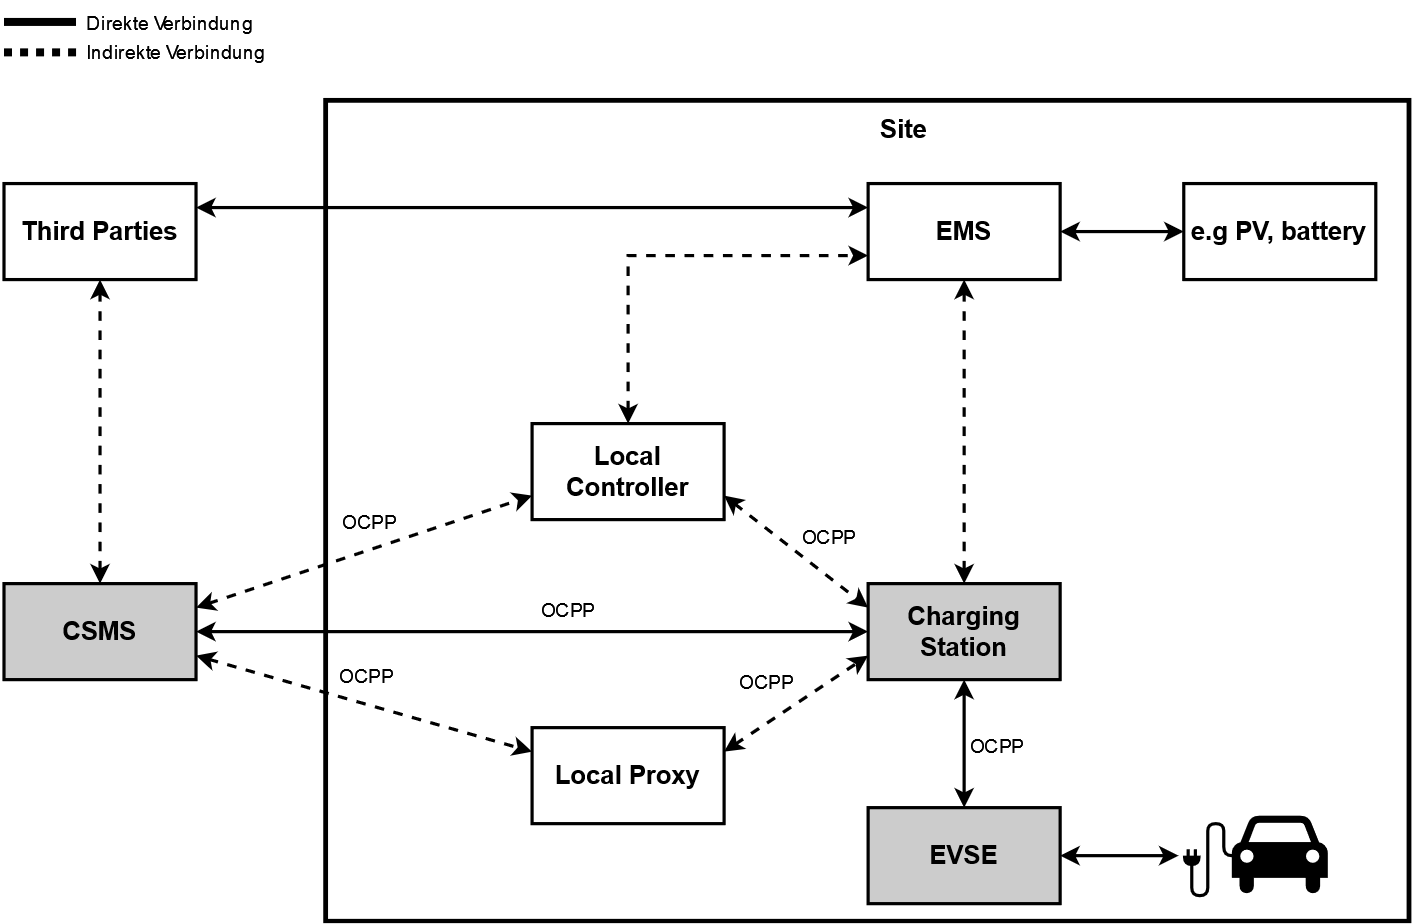
\includegraphics[width=1.0\textwidth]{images/OCPP/Ladesystem.drawio.png}
	\caption{Zusammenhang der Aktuere im \acs{OCPP} Standard \cite{Eigene_Darstellung, ocpp_ieee, OCPP-2.0.1-part1-architecture-topology}}
	\label{fig:Akteure}
\end{figure}

\begin{itemize}
	\item Die Ladesäule (engl. \textit{Charging Station}), ist ein physikalisches System, an dem sich elektrische Fahrzeuge aufladen können. Jede Ladesäule besitzt dabei mindestens ein \textit{\ac{EVSE}}.
	\item Das \acs{EVSE} ist ein individuell verwalteter Teil der Ladesäule, an dem sich immer genau ein elektrisches Fahrzeug aufladen kann.
	\item Das \acs{CSMS} verwaltet die Ladesäulen und kann Benutzer freigeben, eine Ladesäule des Systems zu nutzen.
	\item Das \textit{\ac{EMS}} ist ein Gerät, das den Verbrauch und die Produktion von Energie, auf Basis individueller Einschränkungen oder Vorgaben, verwaltet.
	\item Der \textit{\ac{LP}} ist ein optionales Gerät, welches als Router agiert und mehrere Ladesäulen mit dem \acs{CSMS} über einen Netzwerkknoten kommunizieren lässt. Typischerweise handelt es sich dabei um einen \textit{Managed} oder \textit{Unmanaged} Switch.
	\item Der \textit{\ac{LC}} ist ebenfalls ein optionales Gerät, das im Gegensatz zum \acs{LP} unabhängig vom \acs{CSMS} mit den Ladesäulen kommunizieren kann. Für das \acs{CSMS} agiert es wie eine einzelne Ladesäule. Es wird oft genutzt, um z. B. Ladelimits für die Ladesäulen zu setzen.
	\item Die \textit{Third Parties} stellen in dem Fall andere verwaltende Geräte oder Personen dar, über die das \acs{CSMS} oder \acs{EMS} eingestellt oder verwaltet werden können.
\end{itemize}

\subsubsection{Verbindungsaufbau}\label{OCPP_Websockets}
Damit \acs{CSMS} und Ladesäule über \acs{OCPP} miteinander kommunizieren können, muss vorher eine Verbindung zwischen den Parteien aufgebaut werden. Hierzu verbinden sie sich zuerst über das Websocket Protokoll. Dabei agiert das \acs{CSMS} als Websocket Server und die Ladesäule als WebSocket Client. Die Ladesäule initiiert die Verbindung über einen WebSocket Opening Handshake (siehe \autoref{WebSockets}). Hierbei ist es wichtig, dass in der Endpunkt \ac{URI} eine Nummer oder Bezeichnung enthalten ist, mit dem sich die Ladesäule identifizieren kann. Hierfür wird meistens die vom Hersteller bereitgestellte \ac{ID} der Ladesäule genutzt. Diese wird mit einem \glqq{}/\grqq{} vom Rest der \acfi{URL} getrennt. Zusätzlich muss diese Anfrage im Feld \spverb|Sec-Websocket-Protocol|, die gewünschte OCPP Version enthalten. Die offiziell registrierten Namen sind dabei: ocpp1.6, ocpp2.0.1 etc (vgl. \cite{OCPP-2.0.1-part4-ocpp-j-specification}, S.6). Somit kann die resultierende \acs{HTTP} Request wie in \autoref{lst:opening_handshake} dargestellt aussehen.\\

\begin{lstlisting}[caption={OCPP Opening Handshake Aufbau \cite{Eigene_Darstellung}}, label=lst:opening_handshake, float]
	GET /CSMS/OCPP/EVB28391P HTTP/1.1
	Host: some.server.com:1234
	Upgrade: websocket
	Connection: Upgrade
	Sec-WebSocket-Key: sabkjfhsjksj
	Sec-WebSocket-Protocol: ocpp2.0.1, ocpp1.6
	Sec-WebSocket-Version: 13
\end{lstlisting}

\noindent In diesem Beispiel würde die \textit{ChargePointId} der Ladesäule \glqq{}EVB28391P\grqq{} lauten und sie würde die \acs{OCPP} Version 2.0.1 und 1.6 unterstützen. Dabei würde sie die zuerst genannte Version des Protokolls bevorzugen.

\label{Security_Profiles}
\subsubsection{Security Profiles}
Der oben beschriebene Verbindungsaufbau zwischen \acs{CSMS} und Ladesäule wird entsprechend dem sog. \textit{Security Profile} der beiden Teilnehmer gestartet. Hier wird zwischen verschiedenen Sicherheitsstufen unterschieden:
\begin{itemize}
	\item \textbf{Security Profile 1}: Stellt eine nicht verschlüsselte Verbindung dar, die nur über die \acs{HTTP} \textit{Basic Authentication} geschützt ist. Dies bedeutet, dass der WebSocket Opening Handshake des Clients einen Username und ein Passwort, das Base-64 kodiert ist, enthalten muss. Mit diesem wird sichergestellt, dass sich nur erlaubte Clients mit dem Server verbinden können (vgl. \cite{OCPP-j-1.6-specification}, S.16). Diese Daten werden vom Server ausgewertet und der Handshake nur fortgesetzt, falls diese korrekt sind. Alle anderen ausgetauschten Nachrichten bleiben jedoch unverschlüsselt.
	\item \textbf{Security Profile 2}:
	Der Verbindungsaufbau wird über TLS hergestellt. Dabei braucht nur der Server ein signiertes Zertifikat, das vom Client überprüft wird. Dabei sollte der Client das Root Zertifikat des Servers kennen. Der Client meldet sich weiterhin im Opening Handshake über die \acs{HTTP} Basic Authentication an. Diesmal ist allerdings der Datenverkehr über \acs{TLS} verschlüsselt
	\item \textbf{Security Profile 3}:
	Das Security Profile 3 hat die Besonderheit, dass hier sowohl Client als auch Server ein signiertes Zertifikat benötigen. Beide Zertifikate werden vom jeweils anderen Verbindungspartner überprüft und bei Korrektheit wird eine Verbindung hergestellt. Die \acs{HTTP} Basic Authentication wird hier nicht benötigt, da bereits über das Clientzertifikat sichergestellt ist, dass es sich bereits um einen vertrauenswürdigen Client handelt (vgl. \cite{OCPP-2.0.1-part2-specification-edition2}, S.24ff.). Hier ist ebenfalls jegliche weite Kommunikation verschlüsselt.
\end{itemize}
\subsubsection{\ac{RPC} - Framework}
Sobald eine Websocket Verbindung zwischen dem \acs{CSMS} und  der Ladesäule besteht, werden \acs{OCPP} Nachrichten ausgetauscht. Da die Websocket Verbindung eine Vollduplex Kommunikation zulässt, also Daten gleichzeitig ausgetauscht werden können, ist es nicht möglich Anfragen und Antworten einander zuzuordnen (vgl.\cite{OCPP-2.0.1-part4-ocpp-j-specification}, S.9). Deshalb wird ein zusätzliches Protokoll über der Websocket Schicht benötigt. Hierfür wurde das \acfi{RPC} Protokoll entworfen. Dieses dient als Framework oder \glqq{}Ummantelung\grqq{} der \acs{OCPP} Nachrichten. Im Protokoll wurden dafür drei verschiedene Nachrichtentypen (\verb|MessageTypeID|) definiert:
\begin{itemize}
	\item \textit{Call} entspricht dem Wert 2
	\item \textit{CallResult}  entspricht dem Wert 3
	\item \textit{CallError}  entspricht dem Wert 4
\end{itemize}
Alle Nummern die hier nicht gelistet sind invalide und werden ignoriert.
Die unterschiedlichen Nachrichtentypen haben alle einen eigenen Aufbau, der nun genauer erläutert werden soll:\\

\noindent\textbf{Call}\\
\noindent Die Call Nachricht (siehe \autoref{lst:CALL}) stellt eine Anfrage an einen Teilnehmer dar. Hier enthält die Nachricht immer eine auszuführende Aktion (engl. \textit{Action}). Diese Aktion stellt einen Funktionsaufruf dar und wird im String Format übergeben. Dabei ist der Name dieser gleich eines \acs{OCPP} Befehls. Der Nachricht wird außerdem eine sog.\textit{UniqueId} zugeordnet, welche zur Identifikation benötigt wird. Diese muss unterschiedlich zu allen vorher verwendeten \acs{ID}s sein. Weiter ist noch ein \textit{Payload} im \acfi{JSON} Format enthalten. In diesem sind die zur Nachricht gehörenden \acs{OCPP} Werte enthalten.\\


\begin{lstlisting}[language=json, caption={Call Nachrichten Aufbau \cite{Eigene_Darstellung, OCPP-1.6-edition-2}}, label=lst:CALL, float]
	[<MessageTypeID>,
	"<UniqueID>",
	"<Action>",
	{<Payload>}]
\end{lstlisting}

\noindent Eine Call Nachricht darf nur gesendet werden, falls alle zuvor gesendeten Call Nachrichten bereits von einer \textit{CallResult} oder einer \textit{CallError} Nachricht beantwortet wurden oder eine Call Nachricht eine Zeitüberschreitung hatte. Die Zeitüberschreitung ist dabei allerdings abhängig von der Implementierung des Frameworks, da er frei wählbar ist. Dieser sollte jedoch im Idealfall nach dem Systemaufbau ausgerichtet sein, da z. B. ein Mobilfunk Netzwerk eine längere Übertragungszeit benötigt als ein System, das rein lokal agiert (vgl. \cite{OCPP-2.0.1-part4-ocpp-j-specification}, S.13 ff.).\\

\noindent\textbf{CallResult}\\
\noindent Eine CallResult Nachricht (siehe \autoref{lst:CALLRESULT}) enthält die Antwort zu einer Call Nachricht. Sie wird gesendet, falls die Antwort richtig empfangen und verarbeitet werden konnte. Sie ist ähnlich wie die Call Nachricht aufgebaut, beinhaltet allerdings keine Aktion, da sie nur auf eine Aktion antwortet.
Um zuordnen zu können auf welche Aktion sie antwortet, enthält sie dieselbe uniqueId wie die Call Nachricht. Der \textit{Payload} enthält hier eine Antwort auf die geforderte Aktion bzw. die \acs{OCPP} Nachricht.\\

\begin{lstlisting}[language=json, caption={CallResult Nachrichten Aufbau \cite{Eigene_Darstellung, OCPP-1.6-edition-2}}, label=lst:CALLRESULT, float]
	[<MessageTypeID>,
	"<UniqueID>",
	{<Payload>}]
\end{lstlisting}

\noindent\textbf{CallError}\\
\noindent Falls ein Fehler beim Empfangen der Call Nachricht auftrat oder die Syntax dieser nicht korrekt ist, wird mit einer CallError Nachricht (siehe \autoref{lst:CALLRESULT}) geantwortet (vgl. \cite{OCPP-j-1.6-specification}, S.13). Dabei wird auch kontrolliert, ob die im Payload vorhandenen Daten dem Format der angefragten \acs{OCPP} Nachricht entsprechen. Sie enthält wie die CallResult Nachricht dabei dieselbe uniqueId wie die Call Nachricht. Weiter enthält sie einen errorCode der im Protokoll definiert ist und beschreibt, weshalb die Nachricht nicht verwertet werden konnte. Es ist ebenfalls möglich zu dem errorCode eine Fehlerbeschreibung als String und weitere Details im \acs{JSON} Format anzugeben. Diese sind ebenfalls von der Implementierung abhängig und frei wählbar(vgl. \cite{OCPP-j-1.6-specification}, S.13). Beide Felder können allerdings auch leer gelassen werden bzw. jeweils einen leereren String und ein leeres \acs{JSON} beinhalten.


\begin{lstlisting}[language=json, caption={CallError Nachrichten Aufbau \cite{Eigene_Darstellung, OCPP-1.6-edition-2}}, label=lst:CALLERROR, float]
	[<MessageTypeID>,
	"<UniqueID>",
	"<errorCode>",
	"<errorDescription>",
	{<errorDetails>}]
\end{lstlisting}
\subsubsection{Unterscheidung zwischen OCPP v1.6 und v2.0.1}
Das \acs{OCPP} Protokoll bietet unterschiedliche Versionen an, die sich sehr stark in ihrem Umfang und Nachrichten unterscheiden (vgl. \cite{OCPP-2.0.1-part0-introduction}, S.5ff.). Durch diese Unterschiede ist \acs{OCPP}2.0.1 nicht mehr rückwärts kompatibel mit der Version 1.6. Hier soll darauf eingegangen werden, welche für die Arbeit relevanten Unterschiede in beiden Versionen enthalten sind. Somit wird nicht auf die Unterschiede in Themen \textit{Smart Charging}, \textit{Plug \& Charge} und Benutzerfreundlichkeit eingegangen (siehe \cite{OCPP-2.0.1-part0-introduction}). Stattdessen liegt der Fokus nur beim Thema Transaktionen.\\

%\noindent\textbf{Verwaltung}\\
%\noindent In der \acs{OCPP} Version 2.0.1 wurde das neue sog. \textit{Device Model}(dt. Geräte Model) eingeführt. Vor der Einführung des \textit{Device Model} war es nur möglich, einzelne Konfigurationsparameter der Ladesäule auszulesen und ggf. vor der Verbindung anzupassen. Im neuen \textit{Device Model} ist es nun möglich, einzelne Bauteile der Ladesäule zu erkennen und sich auf Basis dieser ein Modell der Ladesäule aufzubauen. In diesem Model sind alle Komponenten aufgeteilt in drei über Kategorien: der Ladesäule selbst(\textit{Charging Station}), dem \acs{EVSE} und dem \textit{Connector}. Die Komponenten der Ladesäule werden entsprechend dieser Kategorien eingeteilt. Ein Beispiel wie eine typische Ladesäule im Privatgebrauch aufgebaut sein könnte, ist in \autoref{tab:3_tier_anordnung} zu sehen.
%
%\begin{table}[H]
%	\centering
%	\begin{tabularx}{\textwidth}{|X|X|X|}
	%		\hline	
	%		\textbf{Kategorie Ladesäule} & \textbf{Kategorie \acs{EVSE}} & \textbf{Kategorie Connector}\tabularnewline
	%		\hline
	%		Ladesäule selbst & \acs{EVSE} selbst  & Connector selbst\tabularnewline
	%		\hline
	%		\acs{RFID} Lesegerät & Überstrom Sicherung & Steckerverriegelung\tabularnewline
	%		\hline
	%		Funkverbindung & Kontroll Messung &\tabularnewline
	%		\hline
	%		Steuergerät &  FI-Schalter &\tabularnewline
	%		\hline
	%		& Ladestatus Anzeige & \tabularnewline
	%		\hline
	%	\end{tabularx}
%		\caption{\label{tab:3_tier_anordnung} Komponenten einer typischen Ladesäule im privat Betrieb, eingeordnet nach den drei Kategorien}
%\end{table}
%\noindent Dieser Mechanismus erlaubt es ebenfalls die Werte und Attribute der Komponenten optional zu überwachen um eine genauere Fehlerdiagnose zu geben.\\
%
%\noindent\textbf{Sicherheit}\\
%Wie bereits im Kapitel \autoref{Security_Profiles} Security Profiles beschrieben, gibt es mehrere Sicherheitsstufen im Protokoll. Das Security Profile 3 wurde allerdings erst mit \acs{OCPP} 2.0.1 eingeführt. In \acs{OCPP} 1.6 ist es nur möglich den Datenverkehr mit einem Server Zertifikat zu verschlüsseln.\\ \\
\noindent In \acs{OCPP}1.6 wurden Transaktionsdaten in vier verschieden Nachrichten ausgetauscht: \spverb|StartTransaction| (Transaktion wird gestartet), \spverb|StopTransaction| (Transaktion wird gestoppt), \spverb|MeterValue| (Status zur Energie/Strom Übertragung) und \spverb|StatusNotification| (Status der einzelnen Anschlüsse). Diese wurden in \acs{OCPP} 2.0.1 unter der Nachricht: \spverb|TransactionEvent| zusammengefasst.\\
Die \spverb|StatusNotification| Nachricht bleibt weiterhin bestehen, wird aber nur noch für nicht Transaktion relevante Updates zum Status eines Anschlusses genutzt. Ebenfalls wurden von Version 1.6 zu Version 2.0.1 andere Nachrichten Namen geändert. Für die Arbeit relevant sind dabei nur \spverb|GetConfiguration| (Abfragen von Konfigurationsparametern) und \spverb|ChangeConfiguration| (Setzen von Konfigurationsparametern). Diese wurden zu \spverb|GetVariables| und \spverb|SetVariables| umbenannt. Eine Übersicht der Unterschiede ist in \autoref{tab:OCPP_Nachrichten_unterschiede} zu sehen.
\begin{table}[H]
	\begin{tabularx}{\linewidth}{|X|X|X|}
		\hline
		\textbf{OCPP1.6 Nachricht} & \textbf{OCPP2.0.1 Nachricht}                                               & \textbf{Funktion}                                                                        \\ \hline
		StartTransaction            & \begin{tabular}[c]{@{}l@{}}TransactionEvent\\ (type = Started)\end{tabular} & Starte Transaktion                                                                       \\ \hline
		StopTransaction             & \begin{tabular}[c]{@{}l@{}}TransactionEvent\\ (type = Ended)\end{tabular}   & Stoppe Transaktion                                                                       \\ \hline
		MeterValue                  & \begin{tabular}[c]{@{}l@{}}TransactionEvent\\ (type = Updated)\end{tabular} & Lademenge                                                                                \\ \hline
		StatusNotification          & StatusNotification                                                          & \begin{tabular}[c]{@{}l@{}}Status Änderung \\ außerhalb\\ von Transaktionen\end{tabular} \\ \hline
		StatusNotification          & \begin{tabular}[c]{@{}l@{}}TransactionEvent\\ (type = Updated)\end{tabular} & \begin{tabular}[c]{@{}l@{}}Status Änderung\\  innerhalb\\ von Transaktionen\end{tabular} \\ \hline
		GetConfiguration            & GetVariables                                                                & \begin{tabular}[c]{@{}l@{}}Konfigurationsparameter\\ Abfrage\end{tabular}                \\ \hline
		ChangeConfiguration         & SetVariables                                                                & \begin{tabular}[c]{@{}l@{}}Konfigurationsparameter\\ Setzen\end{tabular}                 \\ \hline
	\end{tabularx}
	\caption{Übersicht der Nachrichten Unterschiede in OCPP1.6 und OCPP2.0.1 \cite{Eigene_Darstellung}}
	\label{tab:OCPP_Nachrichten_unterschiede}
\end{table}
